%%%%%%%%%%%%%%%%%%%%%%%%%%%%%%%%%%%%%%%%%
% Journal Article
% LaTeX Template
% Version 1.4 (15/5/16)
%
% This template has been downloaded from:
% http://www.LaTeXTemplates.com
%
% Original author:
% Frits Wenneker (http://www.howtotex.com) with extensive modifications by
% Vel (vel@LaTeXTemplates.com)
%
% License:
% CC BY-NC-SA 3.0 (http://creativecommons.org/licenses/by-nc-sa/3.0/)
%
%%%%%%%%%%%%%%%%%%%%%%%%%%%%%%%%%%%%%%%%%

%----------------------------------------------------------------------------------------
%	PACKAGES AND OTHER DOCUMENT CONFIGURATIONS
%----------------------------------------------------------------------------------------

\documentclass[twoside,twocolumn]{article}

\usepackage{blindtext} % Package to generate dummy text throughout this template

\usepackage[sc]{mathpazo} % Use the Palatino font
\usepackage[T1]{fontenc} % Use 8-bit encoding that has 256 glyphs
\linespread{1.05} % Line spacing - Palatino needs more space between lines
\usepackage{microtype} % Slightly tweak font spacing for aesthetics

\usepackage[english]{babel} % Language hyphenation and typographical rules
\usepackage{graphicx}

\usepackage[hmarginratio=1:1,top=32mm,columnsep=20pt]{geometry} % Document margins
\usepackage[hang, small,labelfont=bf,up,textfont=it,up]{caption} % Custom captions under/above floats in tables or figures
\usepackage{booktabs} % Horizontal rules in tables

\usepackage{lettrine} % The lettrine is the first enlarged letter at the beginning of the text
\usepackage{algorithm}
\usepackage[noend]{algpseudocode}
\usepackage{amsmath}

\usepackage{todonotes}

\usepackage{enumitem} % Customized lists
\setlist[itemize]{noitemsep} % Make itemize lists more compact

\usepackage{abstract} % Allows abstract customization
\renewcommand{\abstractnamefont}{\normalfont\bfseries} % Set the "Abstract" text to bold
\renewcommand{\abstracttextfont}{\normalfont\small\itshape} % Set the abstract itself to small italic text

\usepackage{titlesec} % Allows customization of titles
\renewcommand\thesection{\Roman{section}} % Roman numerals for the sections
\renewcommand\thesubsection{\roman{subsection}} % roman numerals for subsections
\titleformat{\section}[block]{\large\scshape\centering}{\thesection.}{1em}{} % Change the look of the section titles
\titleformat{\subsection}[block]{\large}{\thesubsection.}{1em}{} % Change the look of the section titles

\usepackage{fancyhdr} % Headers and footers
\pagestyle{fancy} % All pages have headers and footers
\fancyhead{} % Blank out the default header
\fancyfoot{} % Blank out the default footer
\fancyhead[C]{Bayesian Optimization in Model Predictive Control $\bullet$ Frederic Dlugi $\bullet$ January 2022} % Custom header text
\fancyfoot[RO,LE]{\thepage} % Custom footer text

\usepackage{titling} % Customizing the title section

\usepackage{hyperref} % For hyperlinks in the PDF

%----------------------------------------------------------------------------------------
%	TITLE SECTION
%----------------------------------------------------------------------------------------

\setlength{\droptitle}{-4\baselineskip} % Move the title up

\pretitle{\begin{center}\Huge\bfseries} % Article title formatting
\posttitle{\end{center}} % Article title closing formatting
\title{Bayesian Optimization in Model Predictive Control} % Article title
\author{%
\textsc{Frederic Dlugi}\\[1ex] % Your name
\normalsize Universität zu Lübeck \\ % Your institution
\normalsize \href{mailto:frederic.dlugi@student.uni-luebeck.de}{frederic.dlugi@student.uni-luebeck.de} % Your email address
%\and % Uncomment if 2 authors are required, duplicate these 4 lines if more
%\textsc{Jane Smith}\thanks{Corresponding author} \\[1ex] % Second author's name
%\normalsize University of Utah \\ % Second author's institution
%\normalsize \href{mailto:jane@smith.com}{jane@smith.com} % Second author's email address
}
\date{\today} % Leave empty to omit a date
\renewcommand{\maketitlehookd}{%
\begin{abstract}
\noindent When using MPC to control a vehicle it is often necessary to fine tune control and vehicle parameters to get good performance in reality. This is a time consuming process that often relies on trial and error or grid search of the parameter space. In this paper we evaluate the use of Bayesian Optimization to tackle this problem. We simulate vehicle dynamics of a simple bicycle model with two parameters. We try to find the MPC cost ratios and real vehicle parameters by optimizing controller performance with different parameters using Bayesian Optimization.
\end{abstract}
}

%----------------------------------------------------------------------------------------

\begin{document}

% Print the title
\maketitle

%----------------------------------------------------------------------------------------
%	ARTICLE CONTENTS
%----------------------------------------------------------------------------------------

\section{Introduction}

\lettrine[nindent=0em,lines=3]{W} e start by introducing bayesian optimization and MPC on a high level.
This is done to let you know what I understand when talking about these algorithms.

\subsection{What is Bayesian Optimization?}
Bayesian optimization is a strategy for global optimization of black-box functions. (Alg. \ref{alg:bo})
It therefore does not require the computation of gradients, but works best on continuous functions.
It is best suited for optimizing functions, where each evaluation takes a long time.
The number of input dimensions for bayesian optimization is typically less then $20$ \cite{frazier2018tutorial}.
Bayesian Optimization uses an acquisition function that operates on a gaussian process of the evaluations. In this paper we evaluate three different acquisition functions: Expected Improvement (Alg. \ref{alg:ei}), Probability of Improvement (Alg. \ref{alg:poi}) and Upper Confidence Bound (Alg. \ref{alg:ucb}). We use the Matern ($\nu=2.5$) kernel for all experiments. We also vary the $\alpha$ Parameter of the Gaussian Process to smooth out the cost landscape.

\begin{algorithm}
    \caption{Bayesian Optimization}
    \label{alg:bo}
    \begin{algorithmic}
        \State $\text{f} \gets \text{black box function}$
        \State $\text{initPos} \gets \text{initial positions}$
        \State $\text{evaluations} \gets \text{f(initPos)}$
        \For{$i= 1 \to N$}
            \State $\alpha \gets \text{acquisitionFunction(evaluations)}$
            \State $\text{nextPos} \gets \text{argmax(}\alpha\text{)}$
            \State $\text{evaluations}.append(\text{f(nextPos)})$
        \EndFor
        \State $result \gets \text{max(evaluations)}$
    \end{algorithmic}
\end{algorithm}

\begin{algorithm}
    \caption{Expected Improvement}
    \label{alg:ei}
    \begin{algorithmic}
        \State $\mu, \sigma \gets \text{gp.predict(x)}$
        \State $z \gets (\mu - y_{max} - \xi)/\sigma$
        \State $result \gets (\mu - y_{max} - \xi) * \text{cdf(z)} + \sigma * \text{pdf(z)}$
    \end{algorithmic}
\end{algorithm}

\begin{algorithm}
    \caption{Probability of Improvement}
    \label{alg:poi}
    \begin{algorithmic}
        \State $\mu, \sigma \gets \text{gp.predict(x)}$
        \State $z \gets (\mu - y_{max} - \xi)/\sigma$
        \State $result \gets \text{cdf(z)}$
    \end{algorithmic}
\end{algorithm}

\begin{algorithm}
    \caption{Upper Confidence Bound}
    \label{alg:ucb}
    \begin{algorithmic}
        \State $\mu, \sigma \gets \text{gp.predict(x)}$
        \State $result \gets \mu + \kappa * \sigma$
    \end{algorithmic}
\end{algorithm}

\subsection{What is MPC?}
MPC is an acronym for model predictive control.
It replaces classical control algorithms that usually work in an offline manner with an optimizer, that solves the optimal control problem for a receding horizon (Figure \ref{fig:mpc}).
Each action taken is the first action of the optimal control plan.
The plan gets updated continuously (Figure \ref{fig:mpc_plan}), this is called receding horizon approach.

\begin{figure}[h]
    \caption{Block-diagram of MPC algorithm}
    \centering
    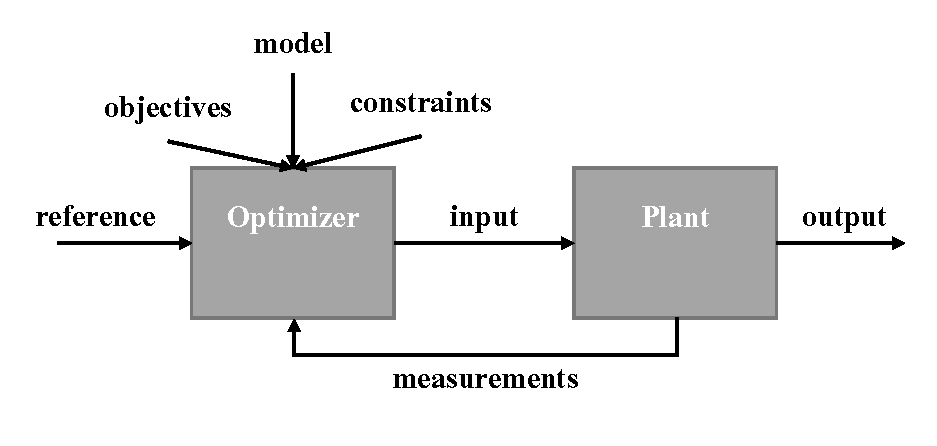
\includegraphics[width=0.45\textwidth]{fig_mpc.pdf}
    \label{fig:mpc}
\end{figure}

\begin{figure}[h]
    \caption{Plan horizon of MPC algorithm}
    \centering
    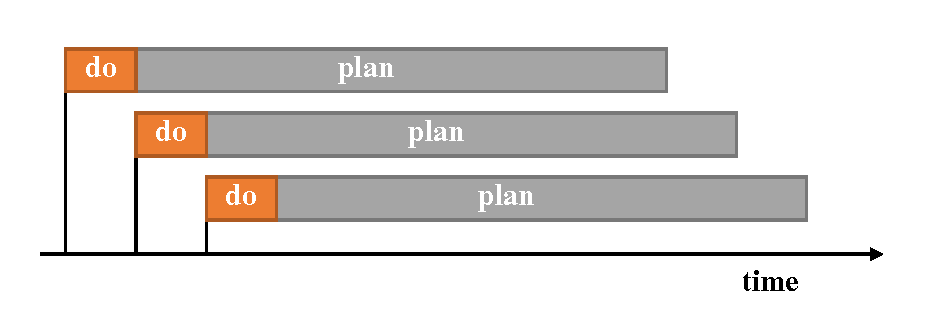
\includegraphics[width=0.45\textwidth]{fig_mpc_plan.pdf}
    \label{fig:mpc_plan}
\end{figure}

\subsection{Kinematic Bicycle Model}

We use a kinematic bicycle model defined by algorithm \ref{alg:kbm} and \ref{alg:ubm} \cite{kinematicBicycleModel}. We try to estimate the $L_r$ and $L_f$ in this paper.
\begin{algorithm}
    \caption{Kinematic Bicycle Model}
    \label{alg:kbm}
    \begin{algorithmic}
        \State $a \gets \text{accelaration (input)}$
        \State $\omega \gets \text{steering angle rate (input)}$
        \State $x_c, y_c \gets \text{center position}$
        \State $v \gets \text{speed}$
        \State $\theta \gets \text{absolute angle}$
        \State $\delta \gets \text{steering angle}$
        \State $\beta \gets \text{side slip factor}$
        \State $L_r \gets \text{Distance center to rear wheel}$
        \State $L_f \gets \text{Distance center to font wheel}$
        \State $L \gets L_r + L_f$
    \end{algorithmic}
\end{algorithm}

\begin{algorithm}
    \caption{Update Bicycle Model}
    \label{alg:ubm}
    \begin{algorithmic}[1]
        \State $\dot{v} \gets a$
        \State $\dot{x_c} \gets v * \cos{(\theta + \beta)}$
        \State $\dot{y_c} \gets v * \sin{(\theta + \beta)}$
        \State $\dot{\theta} \gets v * \cos{(\beta)} * \tan{(\delta)} / L$
        \State $\dot{\delta} \gets \omega$
        \State $\beta \gets \text{atan2}(L_r * \tan{(\delta)}, L)$
    \end{algorithmic}
\end{algorithm}

\section{Literature review}
In Multi-Objective Optimization of a Path-following MPC for Vehicle Guidance \cite{gharib2021multi} BO is used to weight error terms to find the ratio results in the best reference tracking performance of a complex vehicle model in a simulation. Using BO with expected improvement as acquisition function. They found the BO algorithm used to be more efficient then random search when comparing the number of evaluations needed to find satisfactory results.

Lukas Hewing and collaborators \cite{hewing2018cautious} explored the use of BO to decrease model mismatch. They learned a dynamics model of a miniature race car using a gaussian process from real data, while the vehicle is controlled through MPC. They experimented with sparse approximations to gaussian processes to use them in real-time applications.

Lu Qiugang and collaborators \cite{lu2020mpc} explored MPC parameter tuning in HVAC plants. They had good results and with limited evaluations. They used upper confidence bound as acquisition function and also had two tuning parameters. The experiment setup is similar to the one used in this paper.


\section{Experiments}

In this paper we explore two uses of BO in the MPC context. First we try to find the optimal ratio between input (acceleration and steering angle rate) cost and reference tracking ($x - x_{ref}$ and $y - y_{ref}$). Secondly we try to find vehicle specific parameters using BO.

\subsection{Experiment setup}

We explore two uses of BO for MPC. Firstly we try to find the optimal ratio of input cost to state cost ratio (See Fig. \ref{fig:ratio_experiment}). Secondly we estimate $L_r$ and $L_f$ parameters of our controller (See Fig. \ref{fig:l_value_experiment}).

\begin{figure}[h]
    \caption{Ratio experiment}
    \centering
    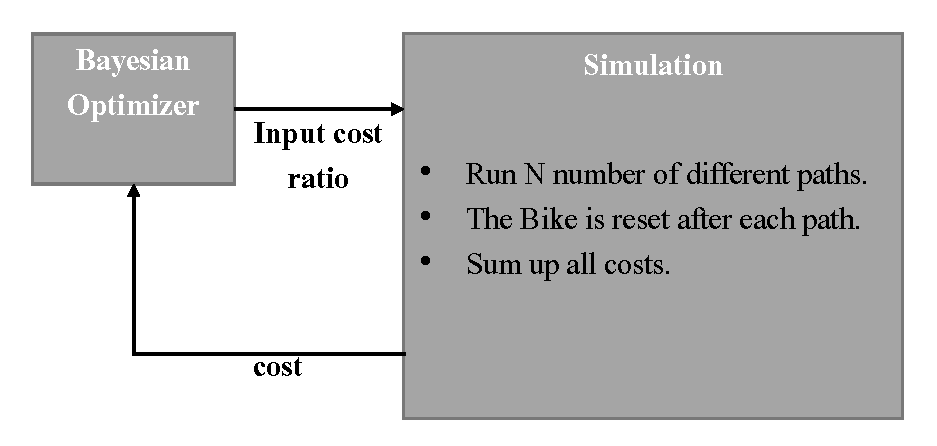
\includegraphics[width=0.45\textwidth]{fig_ratio_experiment.pdf}
    \label{fig:ratio_experiment}
\end{figure}

\begin{figure}[h]
    \caption{L-Value experiment}
    \centering
    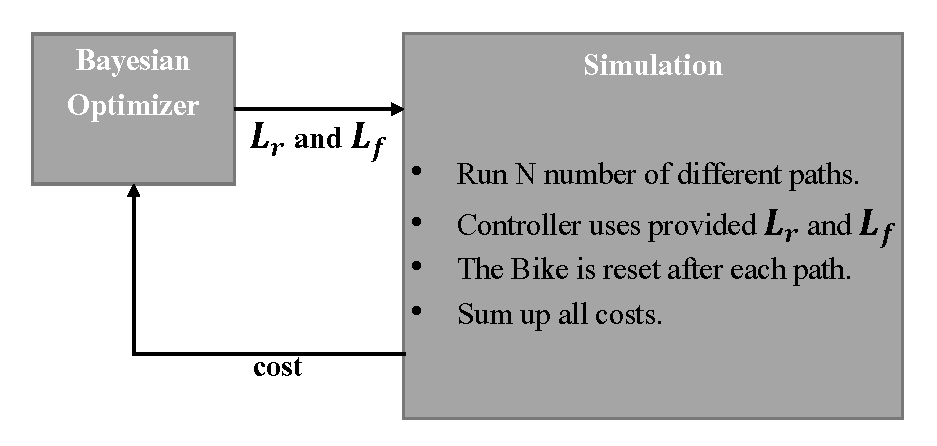
\includegraphics[width=0.45\textwidth]{fig_l_value_experiment.pdf}
    \label{fig:l_value_experiment}
\end{figure}

We used a standard MPC implementation that uses the cost function that is specified here (Alg. \ref{alg:cost_function}). We use scipy's SLSQP optimizer to minimize the cost function.
\begin{algorithm}
    \caption{Cost function}
    \label{alg:cost_function}
    \begin{algorithmic}
        \State $U \gets \text{Array of inputs } (N \times 2)$
        \State $X \gets \text{Array of postions } (N \times 2)$
        \State $X_{ref} \gets \text{Array of reference postions } (N \times 2)$

        \For{$i = 0 \to (N-1)$}
            \State $cost + (X[i] - X_{ref}[i])^T Q (X[i] - X_{ref}[i])$
            \State $cost + U[i]^T R U[i]$
        \EndFor
        \State $return \text{ cost}$
    \end{algorithmic}
\end{algorithm}

To generate the path, we first generate random normal distributed inputs. Then we use the Bicycle model with real $L_r$ and $L_f$ values with these inputs to generate $N$ sequential positions (See Alg. \ref{alg:path_gen}). We use $200$ steps for all paths and all experiments.
\begin{algorithm}
    \caption{Generate Path}
    \label{alg:path_gen}
    \begin{algorithmic}
        \State $L_r \gets \text{Distance center to rear wheel}$
        \State $L_f \gets \text{Distance center to font wheel}$
        \State $\text{initPos} \gets (0,0)$
        \State $\text{N} \gets \text{Number of path points}$
        \State $\text{bike} \gets \text{Bike(}L_r, L_f, \text{initPos}\text{)}$
        \State $\text{inputs} \gets normalDistibutedArray(N - 1, 2)$
        \State $\text{path} \gets zeroArray(N, 2)$
        \For{$i= 1 \to (N-1)$}
            \State $\text{bike}.step(\text{inputs[i - 1]})$
            \State $\text{path[i]} \gets \text{bike}.getPosition()$
        \EndFor
        \State $return \text{ path}$
    \end{algorithmic}
\end{algorithm}

\subsection{Exploring MPC cost ratio using BO}

In this experiment we aim to find the optimal ratio between the $Q$ and $R$ matrix in the cost function (Alg \ref{alg:cost_function}). We try this for different vehicles that are differentiated in their L-parameter. Since a full search of the ratios shows that Ratios between $0.001$ and $0.003$ result in better performance (See Figure \ref{fig:cost_ratio_full}). Therefore we explore only this range in all further experiments. We use $40$ tracks per step and do $30$ steps for both experiments. Increasing the regularization $\alpha$ parameter of the internal GP for BO to $0.01$ improved performance.

\begin{figure}[h]
    \caption{GP of full cost ratio search (Higher is better)}
    \centering
    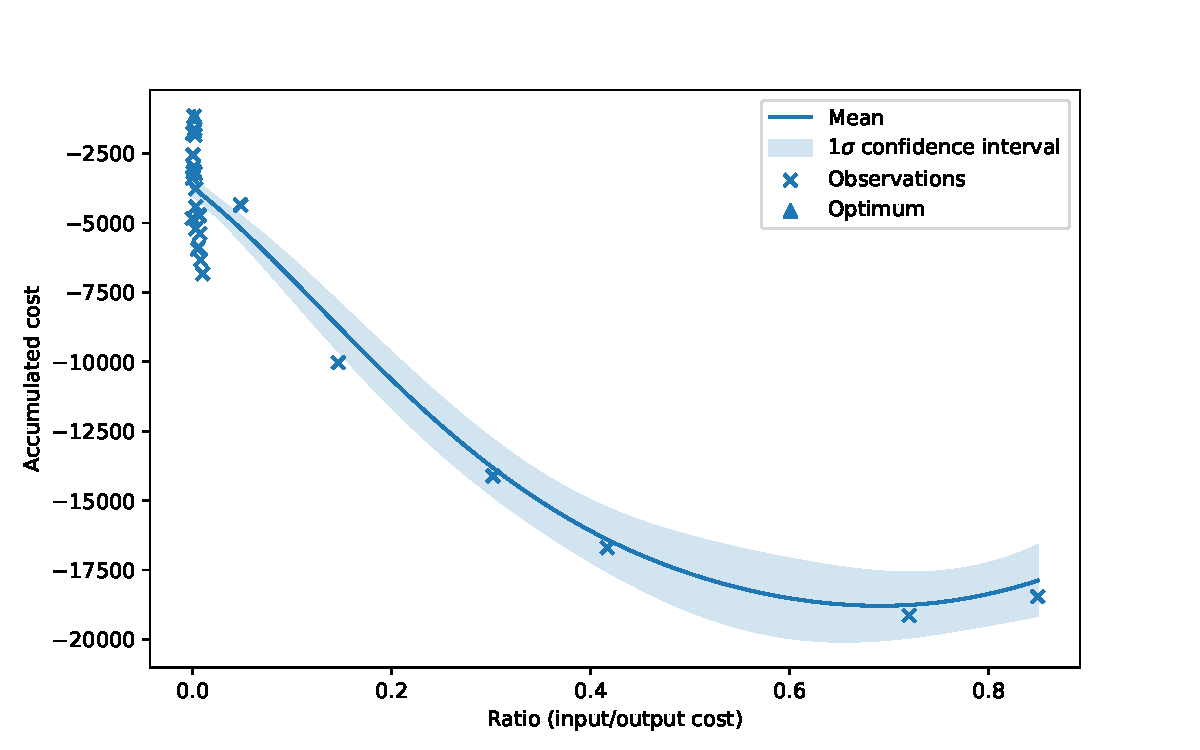
\includegraphics[width=0.45\textwidth]{fig_cost_ratio_full.pdf}
    \label{fig:cost_ratio_full}
\end{figure}

\begin{figure}[h]
    \caption{GP of detailed cost ratio search (Higher is better)}
    \centering
    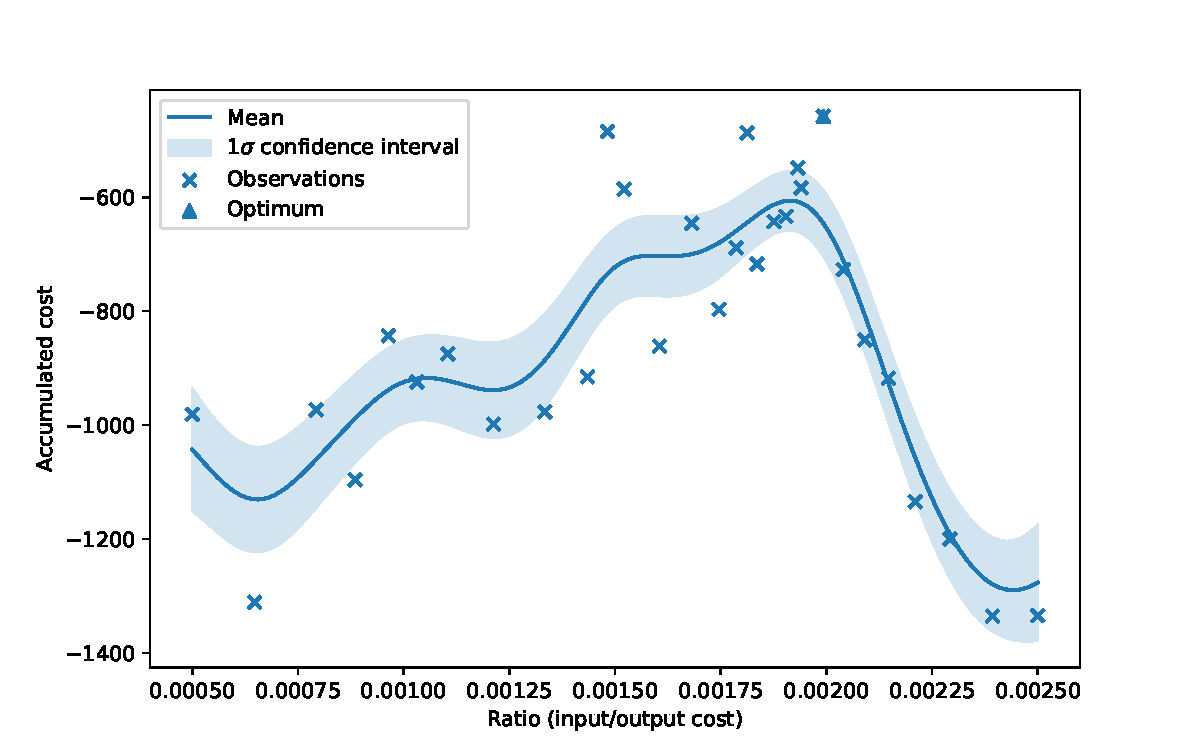
\includegraphics[width=0.45\textwidth]{fig_cost_ratio_detail.pdf}
    \label{fig:cost_ratio_detail}
\end{figure}

We found that the optimum ratio for all tested vehicles all with a length of $2m$ is close to $0.002$ (See Fig \ref{fig:cost_ratio_detail}). This is highly depended on the MPC implementation and vehicle dynamics.

\subsection{Finding Vehicle parameters using BO}

We aim to find the vehicle specific parameters $L_f$ and $L_r$ using BO. We try multiple parameters and different acquisition functions. Since evaluating $40$ tracks still lead to noisy cost we need to choose a suitable exploration-exploitation parameter in our acquisition function. For Expected Improvement \ref{alg:ei} and Probability of Improvement \ref{alg:poi} a $\xi = 0.5$ worked the best. For Upper Confidence Bound a $\kappa=2.576$ worked the best. Increasing the regularization $\alpha$ parameter of the internal GP for BO to $0.1$ improved performance.

\begin{figure}[h]
    \caption{Mean of GP from L-parameter search (Target $L_f = 0.8$ $L_r = 1.2$)}
    \centering
    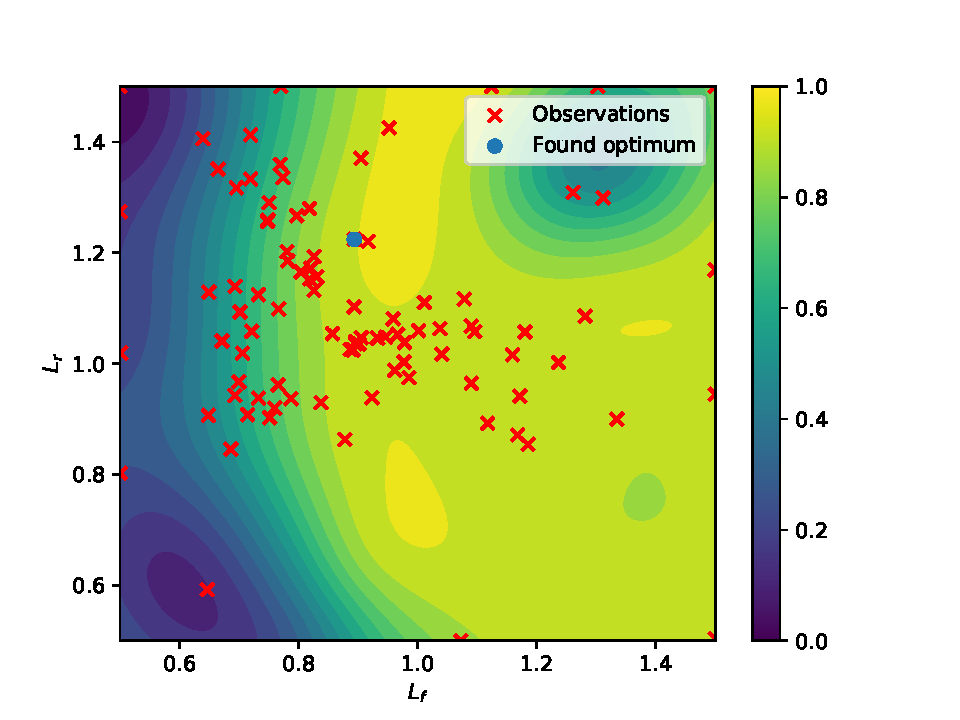
\includegraphics[width=0.45\textwidth]{fig_l_estimation_full.pdf}
    \label{fig:l_param_full}
\end{figure}

\section{Conclusion and further research}
There is no general ratio between input and reference cost. It depends on vehicle dynamics vehicle parameters and the specific MPC implementation. The optimal ratio are still similar and close to $0.002$ with our experiment. Therefore fine tuning is still required and using many different reference tracks, leads to better results.

Finding the vehicle parameters works well using BO if you tweak the BO parameter for exploration and exploitation tradeoff and set the regularization parameter of the internal GP for the BO to a suitable value. Since we only estimated two parameters in our experiment using BO in this case was not helpful.

In further research we would use a more sophisticated MPC since using the SLSQP optimizer from python does not work well for some states. It would also be interesting to try to find more vehicle parameters. Also we would like to try if the BO approach works on real hardware or using one simple and one complex vehicle model this could also be done in simulation by using different vehicle models for the controller and the simulation. In this paper we always measure the current vehicle position and update this inside the controller therefore measuring more or less vehicle states and the effects on the optimization performance would be interesting. To translate this approach to a real vehicle you would need to add uncertainly to measurements and to the model.

\bibliographystyle{plain}
\bibliography{refs.bib}

\end{document}
